\graphicspath{ {./Images/} }

\chapter{Background}

We are going to discuss the basic concepts of this project, both Computer Science and Bioinformatic part. There will
also be a review of different kind of algorithms that are used to solve Sequence Alignment, as well as what is the 
Longest Common Subsequence (LCS) and how is this related to each other. 

\section{P and NP Problem}

The P vs NP problem we are familiar with today was systematically formulated by Stephen Cook in ``The complexity of theorem'' 
proving procedures in 1971. The existing answers to this question are richly described under the framework established 
by Cook. But what is rarely mentioned is that the earliest establishment of the P vs NP problem in history can be
traced back to a letter written by Kurt Gödel to John von Neumann on the hospital bed in 1956 to relieve his boredom.


\subsection{Time-Space Complexity}

Algorithms constitute the basic unit of computer problem-solving, and the execution of each algorithm requires time 
and space. Generally, the larger the input scale, the more time and space is often required. For example, to count 
the traffic of an e-commerce website, the larger the amount of data, the more time it takes.

Therefore, when we are considering the computing time that will be affected by the computer hardware, operating system,
and machine running status at that time, we also need to avoid these effects when we decide if an algorithm is good or not.
Although the execution time of the algorithm is different in different dimensions, the relationship between the input size 
and the growth of time is always constant. If the input scale is represented by N, then the relationship between time T 
and N is usually represented by a curve.

\begin{figure}[h]
    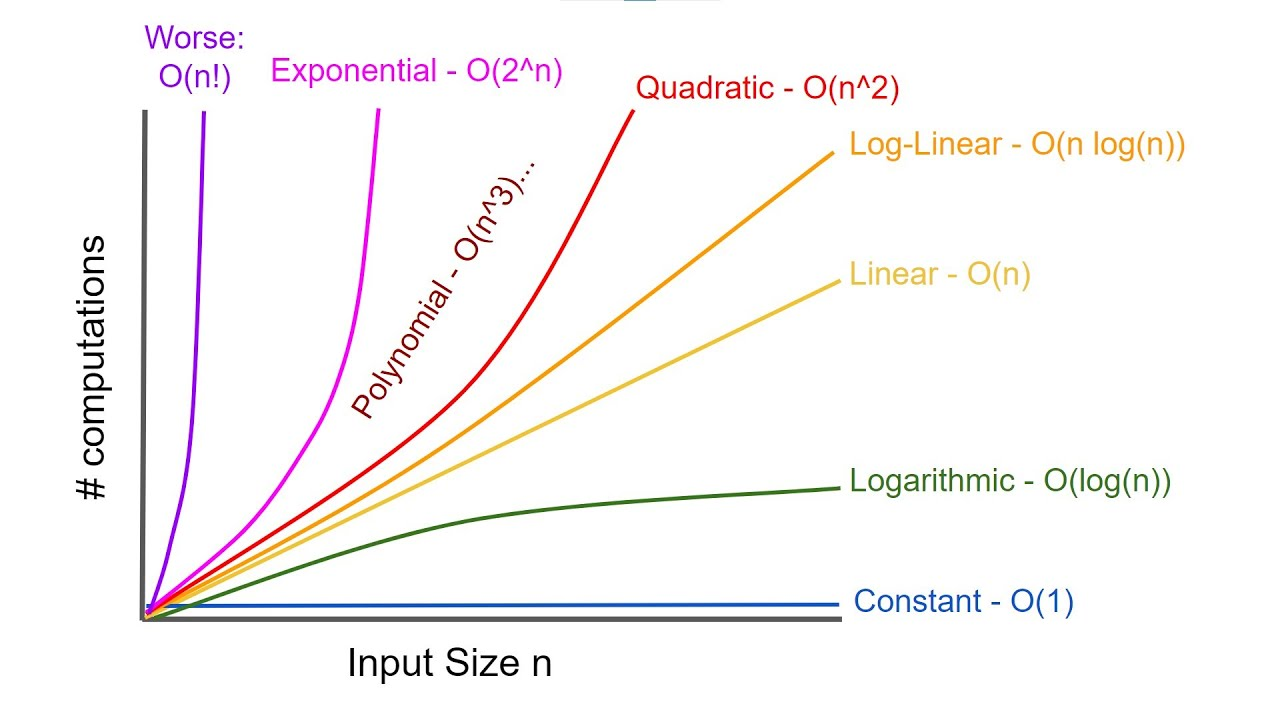
\includegraphics[scale=0.3]{timeComplexity.jpg}
    \caption{A Graphical view of Time Complexity}
    \centering
\end{figure}

The notation O in the graphic is an asymptotic notation to represent the worst-time complexity of a function, the function
inside the O is function that dominates the time complexity of a problem.
\begin{align}
f(x) &= O(g(n))
\end{align}
In the function above, the function $f$ is dominated by $g$. 
Now, we can finally enter into what is actually polynomial time. In terms of mathematical description, it can be described as
this: \[m(n) = O(n^k)\]

Where k is a constant value. It is possible to build a Deterministic Turing Machine to represent these types of functions,
which is one of the main aspects to differentiate P and NP. Since problems that have the worst time-complexity worse than the 
function above may not seem possible to be represented in a Deterministic Turing Machine, but it is known that there is a 
Non-deterministic Turing Machine that represents it, therefore, Non-deterministic polynomial (NP) time.



\subsection{P vs NP}

Following the previous section, there's a clearer way to differentiate P and NP problems, maybe solving a NP problem might be 
a huge task to solve, but to prove that the answer provided is indeed the right answer is easy, actually it's a polynomial time
problem to identify the correctness of a NP problem. For example, solving a Sudoku seems really hard, but proving that it is indeed  
correct is easy, even using a brute-force iteration, the time-complexity would just be $O(n^2)$. 

Actually we can group all P problems as NP problems. That is to say, if a problem can be solved in polynomial time, the solution of a 
problem  must be able to be verified in polynomial time, if all correct solutions have come out, verifying any given solution only 
needs to be compared. The point is, one wonders whether all NP problems are P problems. We can again use the point of view of sets 
to illustrate. If all P problems are classified into one set P, and all NP problems are classified into another set NP, then, obviously,
P belongs to NP. Now, all researches on NP problems focus on one question, whether P = NP or not? The so called "P vs NP" is actually 
just one sentence: prove or overthrow  P = NP.

The problem is still unsolved, no one has proved or overthrew this thesis, however, it is generally accepted that P = NP does not hold,  
There is a reason why people so firmly believe that P does not equal NP is that in the process of studying NP problems, a very special 
class of NP problems has been found called NP-complete problems, also known as NPC problems.

\subsection{ NP-Complete Problems}

To talk about NP-Completeness, we need to understand a few concepts. First, reducibility, basically, a problem A can 
be reduced to a problem B means that problem A can be solved with the solution of problem B, or problem A can be 
``turned into'' problem B. In the book of ``Introduction to Algorithms'' gave such an example, there are two problems: 
a linear equation and a quadratic equation. Then we say that the former can be reduced to the latter, which means that 
if you know how to solve a quadratic equation, you must be able to solve a linear equation. 

Problem A is no more difficult than problem B. It's easy to understand. Since problem A can be solved by problem B, 
if the time complexity of B is lower than that of A, then the algorithm of A can be improved to the algorithm of B, 
and the time complexity of the two is still the same. Just as solving a quadratic equation is more difficult than 
solving a linear equation, because the method for solving the former can be used to solve the latter. This concept allows
us to  go futher, because reducibility have an important property: they are transitive. If problem A can be reduced to 
problem B, and problem B can be reduced to problem C, then problem A must be reduced to problem C. 

Therefore, it is possible to say that there exists an NP problem to which all NP problems can be reduced. In other 
words, once this problem is solved, all NP problems are solved. It is unbelievable that this kind of problem exists, 
and what is even more incredible is that there is not only one such problem, there are many, and it is a kind of 
problem. This type of problem is the NP-Complete problem.

The definition of NPC-Problems is easy, first, it has to be an NP problem; then, all NP problems can be reduced to it.
And to prove a NPC-Problem is also straightforward, first, prove that it is actually an NP problem, and then prove 
that one of the known NPC problems can be reduced to it.

To look at it in another way, we can use the concept of NP-hard, a problem L is said to be NP-hard, if any NP problem 
can be polynomially reduced to L. If an NP-hard problem L itself is NP, then L is said to be NP-complete. 

